\documentclass{standalone}
\usepackage{tikz}
\usetikzlibrary{patterns, positioning}
\usetikzlibrary{shapes.misc}
\usepackage[outline]{contour}
\contourlength{1.5pt} 
\usepackage[sfdefault]{ClearSans} %% option 'sfdefault' activates Clear Sans as the default text font
\usepackage[T1]{fontenc}

\begin{document}
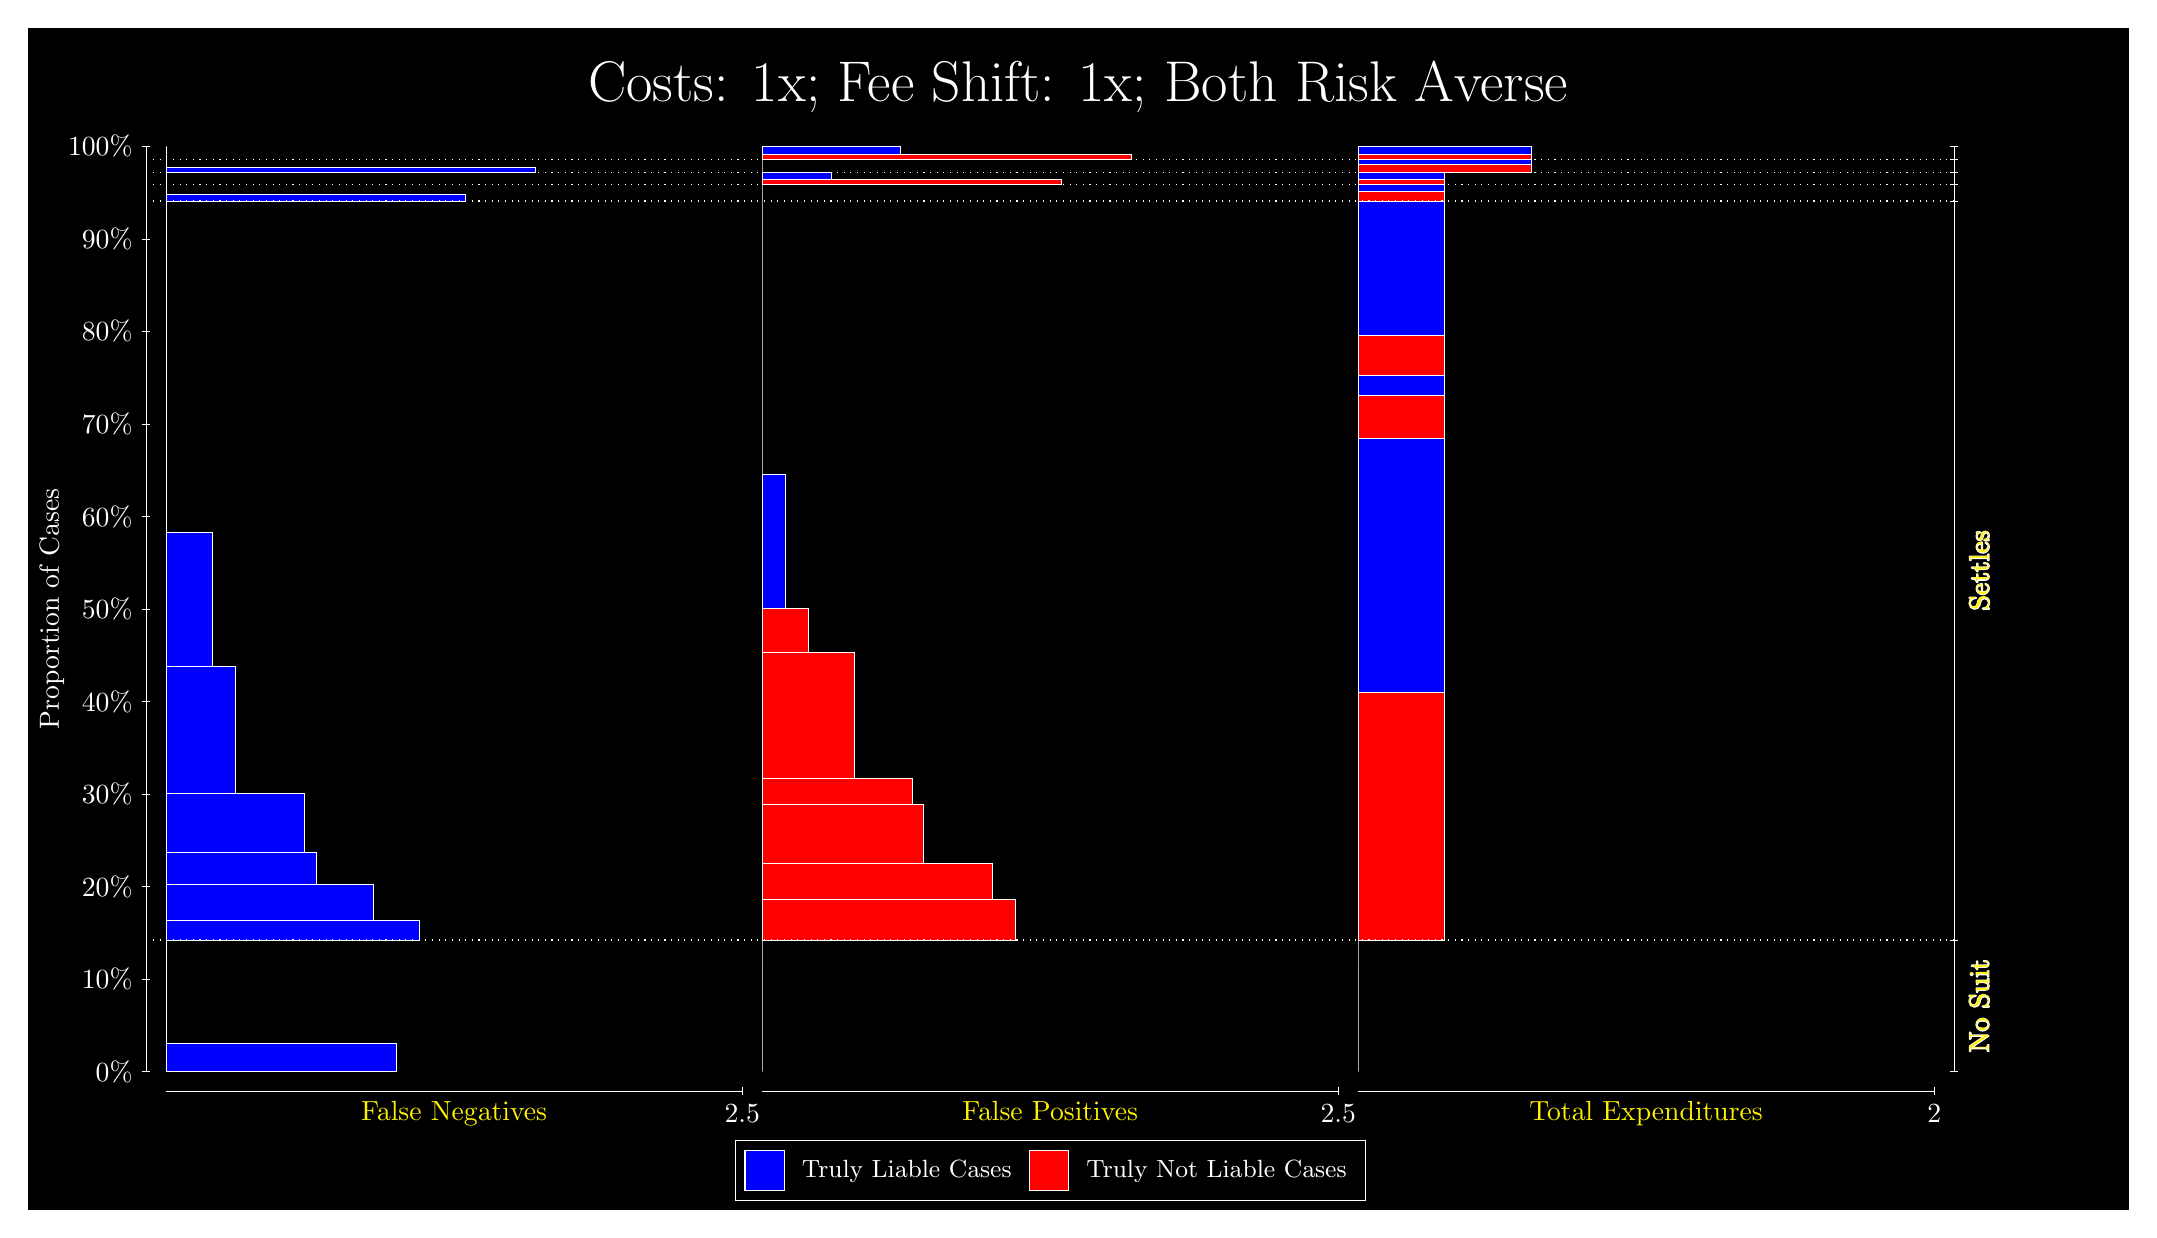
\begin{tikzpicture}
\draw[fill=black] (0,0) rectangle (26.667,15);
\draw[text=white] (0,13.5) rectangle (26.667,15) node[midway] {\huge Costs: 1x; Fee Shift: 1x; Both Risk Averse};
\draw[white, very thin] (1.5,1.75) -- (1.5,13.5);
\node[rotate=90, text=white, anchor=center] at (0.3, 7.625) {Proportion of Cases};
\draw[white, very thin] (1.45,1.75) -- (1.55,1.75);
\node[text=white, anchor=east] at (1.45, 1.75) {0\%};
\draw[white, very thin] (1.45,2.925) -- (1.55,2.925);
\node[text=white, anchor=east] at (1.45, 2.925) {10\%};
\draw[white, very thin] (1.45,4.1) -- (1.55,4.1);
\node[text=white, anchor=east] at (1.45, 4.1) {20\%};
\draw[white, very thin] (1.45,5.275) -- (1.55,5.275);
\node[text=white, anchor=east] at (1.45, 5.275) {30\%};
\draw[white, very thin] (1.45,6.45) -- (1.55,6.45);
\node[text=white, anchor=east] at (1.45, 6.45) {40\%};
\draw[white, very thin] (1.45,7.625) -- (1.55,7.625);
\node[text=white, anchor=east] at (1.45, 7.625) {50\%};
\draw[white, very thin] (1.45,8.8) -- (1.55,8.8);
\node[text=white, anchor=east] at (1.45, 8.8) {60\%};
\draw[white, very thin] (1.45,9.975) -- (1.55,9.975);
\node[text=white, anchor=east] at (1.45, 9.975) {70\%};
\draw[white, very thin] (1.45,11.15) -- (1.55,11.15);
\node[text=white, anchor=east] at (1.45, 11.15) {80\%};
\draw[white, very thin] (1.45,12.325) -- (1.55,12.325);
\node[text=white, anchor=east] at (1.45, 12.325) {90\%};
\draw[white, very thin] (1.45,13.5) -- (1.55,13.5);
\node[text=white, anchor=east] at (1.45, 13.5) {100\%};

\draw[white, very thin] (24.457,1.75) -- (24.457,13.5);
\draw[white, very thin] (24.407,1.75) -- (24.507,1.75);
\node[anchor=west] at (24.407, 1.75) {};
\draw[white, very thin] (24.407,3.4203) -- (24.507,3.4203);
\node[anchor=west] at (24.407, 3.4203) {};
\draw[white, very thin] (24.407,12.806) -- (24.507,12.806);
\node[anchor=west] at (24.407, 12.806) {};
\draw[white, very thin] (24.407,13.016) -- (24.507,13.016);
\node[anchor=west] at (24.407, 13.016) {};
\draw[white, very thin] (24.407,13.171) -- (24.507,13.171);
\node[anchor=west] at (24.407, 13.171) {};
\draw[white, very thin] (24.407,13.332) -- (24.507,13.332);
\node[anchor=west] at (24.407, 13.332) {};
\draw[white, very thin] (24.407,13.5) -- (24.507,13.5);
\node[anchor=west] at (24.407, 13.5) {};

\draw[white, very thin, fill=blue] (1.75,1.75) rectangle (4.6775,2.1082);
\draw[white, very thin, fill=red] (1.75,2.1082) rectangle (1.75,3.4203);
\draw[white, very thin, fill=blue] (1.75,3.4203) rectangle (4.9703,3.6688);
\draw[white, very thin, fill=blue] (1.75,3.6688) rectangle (4.3848,4.1289);
\draw[white, very thin, fill=blue] (1.75,4.1289) rectangle (3.6529,4.5347);
\draw[white, very thin, fill=blue] (1.75,4.5347) rectangle (3.5065,5.2873);
\draw[white, very thin, fill=blue] (1.75,5.2873) rectangle (2.6283,6.8916);
\draw[white, very thin, fill=blue] (1.75,6.8916) rectangle (2.3355,8.5932);
\draw[white, very thin, fill=red] (1.75,8.5932) rectangle (1.75,12.806);
\draw[white, very thin, fill=blue] (1.75,12.806) rectangle (5.5558,12.895);
\draw[white, very thin, fill=red] (1.75,12.895) rectangle (1.75,13.016);
\draw[white, very thin, fill=red] (1.75,13.016) rectangle (1.75,13.083);
\draw[white, very thin, fill=blue] (1.75,13.083) rectangle (1.75,13.171);
\draw[white, very thin, fill=blue] (1.75,13.171) rectangle (6.4341,13.237);
\draw[white, very thin, fill=red] (1.75,13.237) rectangle (1.75,13.332);
\draw[white, very thin, fill=red] (1.75,13.332) rectangle (1.75,13.399);
\draw[white, very thin, fill=blue] (1.75,13.399) rectangle (1.75,13.5);
\draw[white, very thin, fill=red] (9.3189,1.75) rectangle (9.3189,3.0622);
\draw[white, very thin, fill=blue] (9.3189,3.0622) rectangle (9.3189,3.4203);
\draw[white, very thin, fill=red] (9.3189,3.4203) rectangle (12.539,3.9342);
\draw[white, very thin, fill=red] (9.3189,3.9342) rectangle (12.246,4.3943);
\draw[white, very thin, fill=red] (9.3189,4.3943) rectangle (11.368,5.1469);
\draw[white, very thin, fill=red] (9.3189,5.1469) rectangle (11.222,5.4741);
\draw[white, very thin, fill=red] (9.3189,5.4741) rectangle (10.49,7.0785);
\draw[white, very thin, fill=red] (9.3189,7.0785) rectangle (9.9044,7.6337);
\draw[white, very thin, fill=blue] (9.3189,7.6337) rectangle (9.6116,9.3352);
\draw[white, very thin, fill=blue] (9.3189,9.3352) rectangle (9.3189,12.806);
\draw[white, very thin, fill=red] (9.3189,12.806) rectangle (9.3189,12.927);
\draw[white, very thin, fill=blue] (9.3189,12.927) rectangle (9.3189,13.016);
\draw[white, very thin, fill=red] (9.3189,13.016) rectangle (13.125,13.083);
\draw[white, very thin, fill=blue] (9.3189,13.083) rectangle (10.197,13.171);
\draw[white, very thin, fill=red] (9.3189,13.171) rectangle (9.3189,13.266);
\draw[white, very thin, fill=blue] (9.3189,13.266) rectangle (9.3189,13.332);
\draw[white, very thin, fill=red] (9.3189,13.332) rectangle (14.003,13.399);
\draw[white, very thin, fill=blue] (9.3189,13.399) rectangle (11.075,13.5);
\draw[white, very thin, fill=red] (16.888,1.75) rectangle (16.888,3.0622);
\draw[white, very thin, fill=blue] (16.888,3.0622) rectangle (16.888,3.4203);
\draw[white, very thin, fill=red] (16.888,3.4203) rectangle (17.986,6.5646);
\draw[white, very thin, fill=blue] (16.888,6.5646) rectangle (17.986,9.7874);
\draw[white, very thin, fill=red] (16.888,9.7874) rectangle (17.986,10.343);
\draw[white, very thin, fill=blue] (16.888,10.343) rectangle (17.986,10.591);
\draw[white, very thin, fill=red] (16.888,10.591) rectangle (17.986,11.105);
\draw[white, very thin, fill=blue] (16.888,11.105) rectangle (17.986,12.806);
\draw[white, very thin, fill=red] (16.888,12.806) rectangle (17.986,12.927);
\draw[white, very thin, fill=blue] (16.888,12.927) rectangle (17.986,13.016);
\draw[white, very thin, fill=red] (16.888,13.016) rectangle (17.986,13.083);
\draw[white, very thin, fill=blue] (16.888,13.083) rectangle (17.986,13.171);
\draw[white, very thin, fill=red] (16.888,13.171) rectangle (19.083,13.266);
\draw[white, very thin, fill=blue] (16.888,13.266) rectangle (19.083,13.332);
\draw[white, very thin, fill=red] (16.888,13.332) rectangle (19.083,13.399);
\draw[white, very thin, fill=blue] (16.888,13.399) rectangle (19.083,13.5);
\draw[white, dotted] (1.5,3.4203) -- (24.457,3.4203);
\draw[white, dotted] (1.5,12.806) -- (24.457,12.806);
\draw[white, dotted] (1.5,13.016) -- (24.457,13.016);
\draw[white, dotted] (1.5,13.171) -- (24.457,13.171);
\draw[white, dotted] (1.5,13.332) -- (24.457,13.332);
\draw[white, very thin] (1.75,1.5) -- (9.0689,1.5);
\node[text=yellow, anchor=north] at (5.4094, 1.5) {False Negatives};
\draw[white, very thin] (9.0689,1.45) -- (9.0689,1.55);
\node[text=white, anchor=north] at (9.0689, 1.45) {2.5};

\draw[white, very thin] (9.3189,1.5) -- (16.638,1.5);
\node[text=yellow, anchor=north] at (12.978, 1.5) {False Positives};
\draw[white, very thin] (16.638,1.45) -- (16.638,1.55);
\node[text=white, anchor=north] at (16.638, 1.45) {2.5};

\draw[white, very thin] (16.888,1.5) -- (24.207,1.5);
\node[text=yellow, anchor=north] at (20.547, 1.5) {Total Expenditures};
\draw[white, very thin] (24.207,1.45) -- (24.207,1.55);
\node[text=white, anchor=north] at (24.207, 1.45) {2};

\node[text=yellow, centered, rotate=90] at (24.777, 2.5852) {\contour{white}{No Suit}};
\node[text=yellow, centered, rotate=90] at (24.777, 8.1134) {\contour{white}{Settles}};





\draw (12.978300999999998,1.5) node[draw=none] (baseCoordinate) {};
\begin{scope}[align=center]
        \matrix[scale=0.5, draw=white, below=0.5cm of baseCoordinate, nodes={draw}, column sep=0.1cm]{
            \node[rectangle, draw, minimum width=0.5cm, minimum height=0.5cm, fill=blue] {}; &
            \node[draw=none, font=\small, text=white] (B) {Truly Liable Cases}; &
            \node[rectangle, draw, minimum width=0.5cm, minimum height=0.5cm, fill=red] {}; &
            \node[draw=none, font=\small, text=white] (B) {Truly Not Liable Cases}; \\
            };
\end{scope}

\end{tikzpicture}
\end{document}